


\subsection { Implementation in OpenStack Swift}
\label{sec:implementation}

 \begin{figure} [t]
 	\centering
 	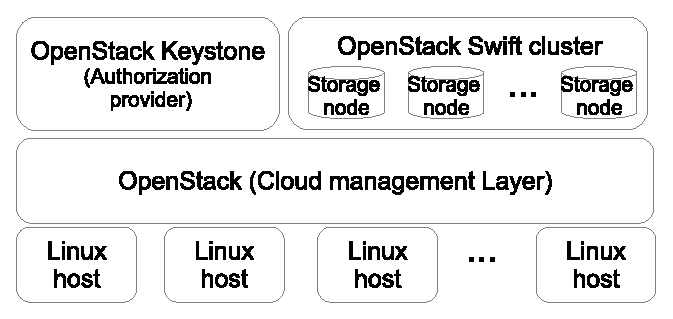
\includegraphics[width=.6\textwidth]{NSS16/reference-implementation-architecture}
 	\caption{Reference architecture of the implementation testbed}
 	\label{fig:reference-implementation-architecture}
 \end{figure}


 
 	\begin{figure} [t]
 		\centering
 		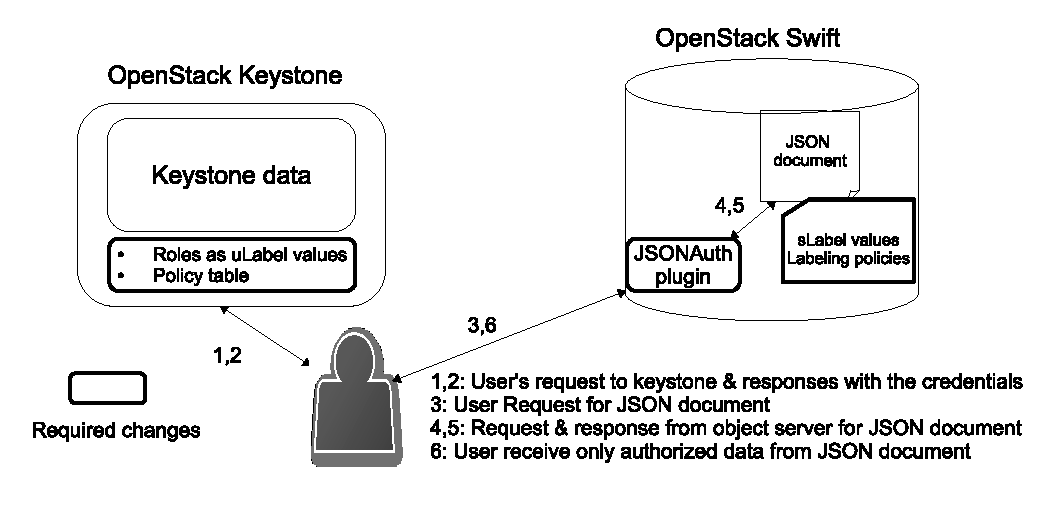
\includegraphics[width=.9\textwidth]{NSS16/implementation-in-swift}
 		\caption{Implementation in OpenStack IaaS cloud platform}
 		\label{fig:implementation-in-swift}
 	\end{figure}
 

We have implemented our proposed operational model and path-based labeling scheme in OpenStack IaaS cloud platform using OpenStack Keystone as the authorization service provider and OpenStack Swift as the storage service provider. Our choice of OpenStack is motivated by its support for independent and inter-operable  services and a well defined RESTful API set.

We have modified OpenStack Keystone and Swift services to accommodate required changes. A reference architecture of our testbed is given in Figure \ref{fig:reference-implementation-architecture}. Details of the implementation is shown in Figure \ref{fig:implementation-in-swift}. Required changes are presented as highlighted rectangles in Figure \ref{fig:implementation-in-swift}.

\subsection{Changes in OpenStack Keystone}

 OpenStack Keystone uses roles and role-based policies to provide authorization decisions. In our implementation, we uses roles to hold user-label attribute values. A set of valid security-label values are also stored as part of the Keystone service.
 
 Among two different types of policies - authorization and labeling policies, the former is managed in the Keystone service. We assume, a higher level administrators (possibly at the level of organization) adds, removes or updates these authorization policies. We add a policy table in Keystone database to store these enumerated authorization policies. 

\subsection{Changes in OpenStack Swift}

In Swift side, we store \textit{security-label} values assigned to JSON objects and path-based labeling policies applied to them.  Security-label values and labeling policies are stored as metadata of the stored objects, JSON documents in this case. For simplicity, we assume object owner (Swift account holder in this case) can update security-label values or labeling policies for stored JSON document. 


 During evaluation, we intercept every requests to Swift (from the Swift-proxy server) and reroute a request to be passed through \textit{JSONAuth plugin} if it is a request for a JSON document. In this case, the request additionally carries a requested path and authorization policies applicable to the user. JSONAuth plug-in retrieves the requested JSON document, apply path-based labeling policies to annotate the document and uses authorization policies to determine if the user is authorized for the requested content of the file. 

\subsection{Evaluation}

 \begin{figure} [t]
 	\centering
 	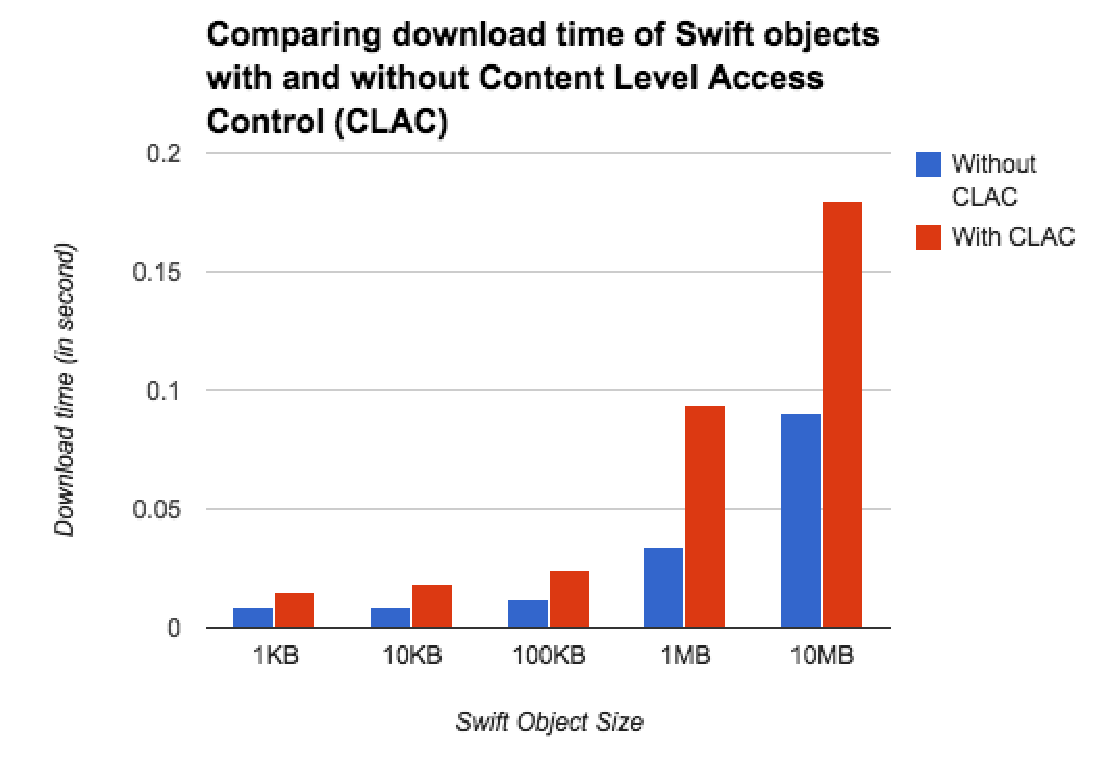
\includegraphics[width=.9\textwidth]{NSS16/performance}
 	\caption{Performance evaluation}
 	\label{fig:performance-a}
 \end{figure}


An evaluation of our implementation is shown in Figure \ref{fig:performance}. The evaluation has been made against concurrent download requests to the Swift proxy server. The X-axis shows size of the JSON document requested for download while the Y-axis shows the average download time for 10 concurrent request. Our evaluation shows a performance hit of nearly 60\% over no authorization protection.
%\textbf{Performance}


